
%
\section{Introduction} % (fold)
\label{sec:pev_introduction}
%
The \ac{PV} operator \cite{Peikert1999} is a generic and
widely spread concept in visualization.
%
Given two \ac{3D} vector fields $ \vv_1, \vv_2$, the \ac{PV} operator delivers all points
in the \ac{3D} domain where $ \vv_1$ and $\vv_2$ are linearly dependent.
%
It is known that the \ac{PV} operator delivers structurally stable lines which we
call \ac{PV} lines.
%
Applying it to different concrete vector fields, the \ac{PV} operator has been
proven to be a generic tool to extract vortex core lines or bifurcation lines.
%
Several numerical methods to extract \ac{PV} lines have been developed.
%
\Todo[inline]{Make chronological connection to tensor core lines (first PEV then
TCL). This algorithm devised first.}
%

%
Recently, Oster \etal \cite{Oster2018} introduced the concept of
{\em tensor core lines}, which represent cores of swirling hyperstreamlines
in tensor fields.
%
These lines are defined as the locations where a (real) eigenvector of the
tensor field is parallel to a (real) eigenvector of the tensor field's
directional derivative in the direction of this eigenvector.
%
In this paper we extend this concept to a more generic formulation: the \ac{PEV}
operator of two (not necessarily symmetric) \ac{3D} second order tensor fields.
%
Let $\mS(\vx)$ and $\mT(\vx)$ be two such tensor fields.
%
Then the \ac{PEV} operator collects all points where $\mS$ and $\mT$ have parallel
real eigenvectors.
%
This can be concisely expressed as
%
\begin{equation}
    \operatorname{PEV}(\mS,\mT) = \{ \vx \;|\; \exists \;\ve,
        \ve \parallel \mS(\vx)\,\ve \parallel \mT(\vx)\,\ve \}\,\text{.}
\end{equation}
%

%
In this chapter, we establish this operator by...
%
\begin{itemize}
    \item
    ... studying its properties.
    %
    In particular, we show that the \ac{PEV} operator produces structurally stable
    line structures.
    %
    \item
    ... presenting a numerical algorithm to extract \ac{PEV} lines in piecewise
    linear tensor fields.
    %
    The main idea is to do a recursive search not only in \ac{3D} space but
    simultaneously in \ac{3D} space and the space of all possible eigenvectors.
    %
    \item
    ... applying it to compare pairs of stress tensor fields defined on the same
    domain.
    %
    % In this way, we are able to find locations where two
    % different loads produce principal stresses aligned in the same direction.
    %
\end{itemize}
%}
%
\subsection*{Relation to the \ac{PV} operator}
\Todo{don't use starred sectioning}
%
At first glance, the \ac{PEV} operator seems to be a straightforward extension of the
classical \ac{PV} operator:
%
given two tensor fields $\mS, \mT$, consider the eigenvector fields as
vector fields and apply the \ac{PV} operator to them.
%
However, as Oster \etal \cite{Oster2018} pointed out, using such a naive
approach would suffer from several problems:
%
\begin{itemize}
    \item
    %
    Interpreting the eigenvectors of a tensor field as a vector field would
    require a heuristic choice of the orientation and magnitude of the vectors.
    %
    This choice can not generally be made in a globally consistent manner.
    %
    \item
    In regions with three real eigenvectors, it is not clear which one to
    choose for a representative vector field.
    %
    \item
    Small changes in a tensor may result in a dramatic change in eigenvector
    direction, or even the sudden appearance or disappearance of real
    eigenvectors.
    %
\end{itemize}
%
All of these problems show that eigenvector fields are fundamentally different
from vector fields, for which the \ac{PV} operator is designed.
%
Extracting \ac{PEV} lines requires new algorithms that are explicitly designed for
tensor fields.
%

%
There are a number of approaches in vortex extraction where a vector field $\vv$
is compared to the eigenvectors of a tensor field $\mS$.
%
This ``mixed case'' (eigenvector parallel to a vector) can be easily reduced to
the classical \ac{PV} operator by comparing $\vv$ and $\mS\,\vv$.
%
The challenging case considered in this paper is the comparison of the
eigenvectors of two tensor fields.

%
In the following, we first give an overview of related work and introduce the
notation used throughout the paper.
%
We then give some theoretical properties of the \ac{PEV} operator in
\cref{sec:pev_theory}, before detailing our algorithm for finding \ac{PEV} lines in
piecewise linear tensor fields in \cref{sec:extracting_pev_lines}.
%
In \cref{sec:pev_results}, we present our results for mechanical stress tensor
data.
%
We close with a discussion and future work in \cref{sec:pev_discussion} and
\cref{sec:pev_limitations}.
%
\begin{figure}[t]
    \centering
    \begin{tikzpicture}
        \node (img1gen) {
            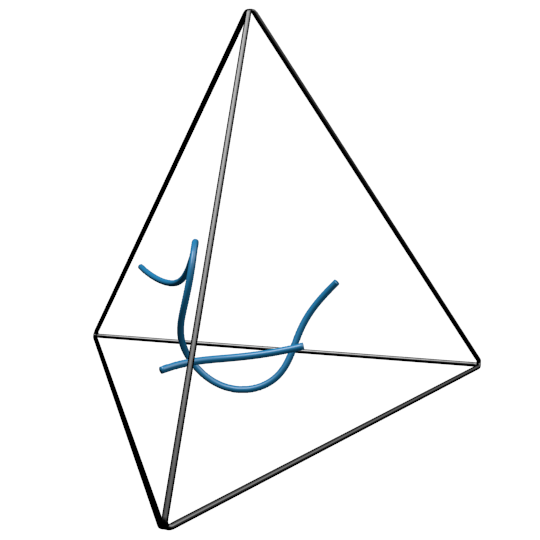
\includegraphics[width=0.3\columnwidth]{figures/Rand_general_1.png}
        };
        \node[right=0pt of img1gen] (img2gen) {
            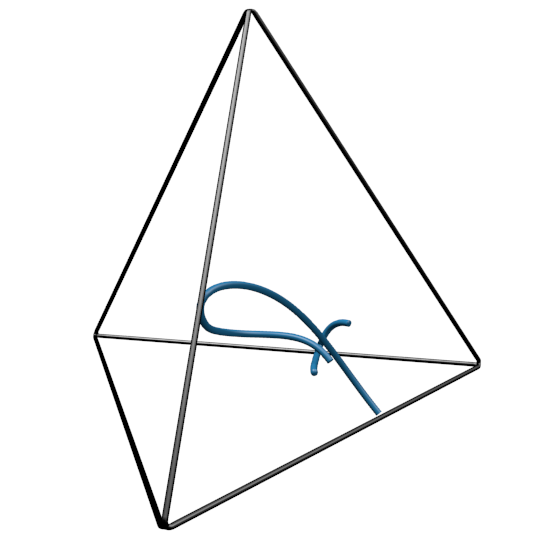
\includegraphics[width=0.3\columnwidth]{figures/Rand_general_3.png}
        };
        \node[right=0pt of img2gen] (img3gen) {
            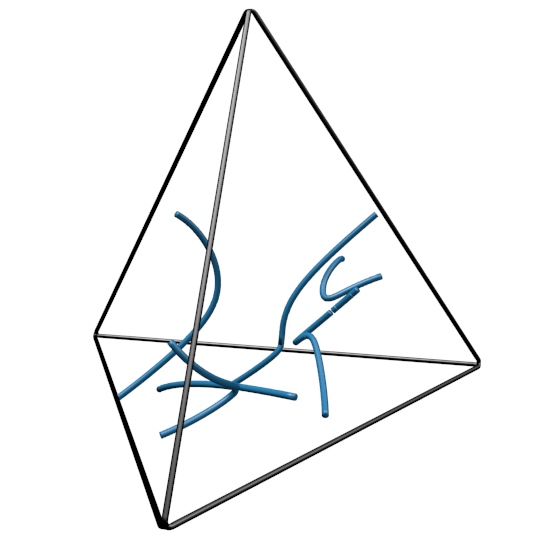
\includegraphics[width=0.3\columnwidth]{figures/Rand_general_4.png}
        };

        \node[below=0pt of img1gen] (img1symm) {
            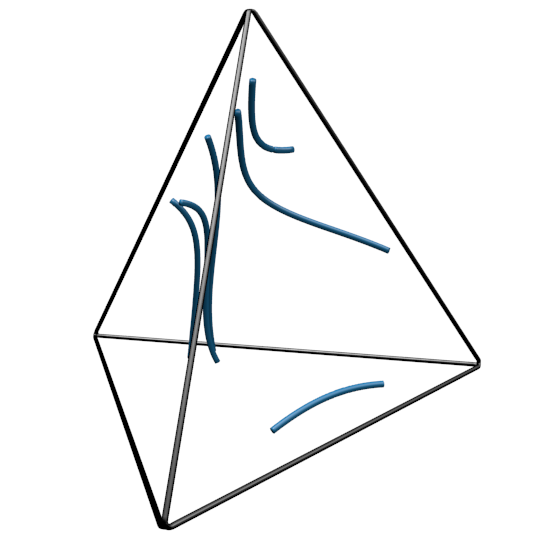
\includegraphics[width=0.3\columnwidth]{figures/Rand_symm_2.png}
        };
        \node[right=0pt of img1symm] (img2symm) {
            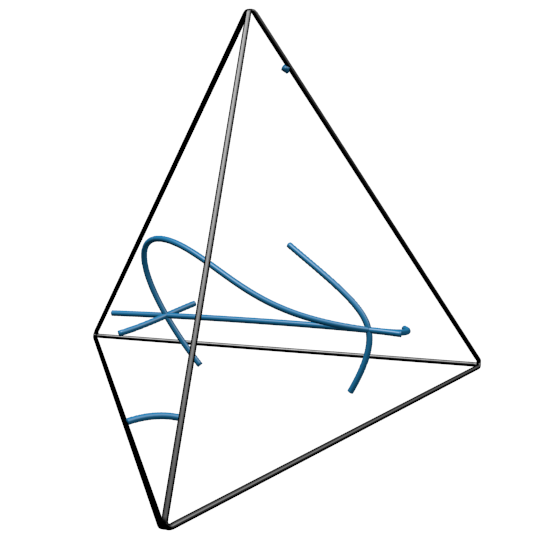
\includegraphics[width=0.3\columnwidth]{figures/Rand_symm_3.png}
        };
        \node[right=0pt of img2symm] (img3symm) {
            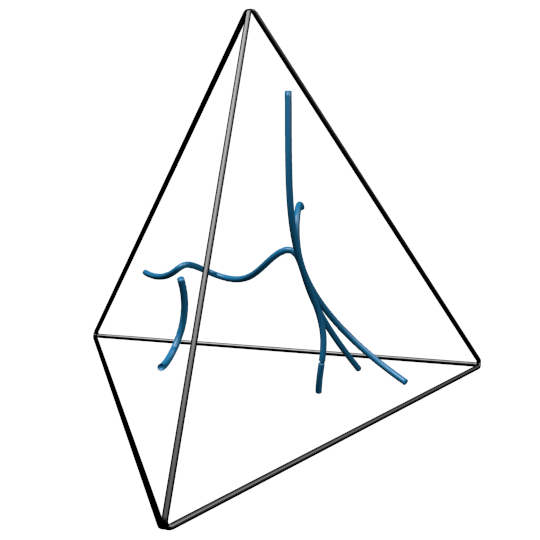
\includegraphics[width=0.3\columnwidth]{figures/Rand_symm_4.png}
        };
    \end{tikzpicture}
    \caption{\ac{PEV} lines in pairs of random linear tensor fields. Top: General
             tensors. Bottom: Symmetric tensors. Symmetric tensors generally
             produce more lines, as they always have three real eigenvectors.
             General tensor \ac{PEV} lines generally do not intersect, while it is
             common for symmetric tensor \ac{PEV} lines to do so. If they do,
             three \ac{PEV} lines always intersect at once, as their eigenvectors
             are orthogonal.}
    \label{fig:rand_lines}
\end{figure}
%
%
% section introduction (end)